% !TeX spellcheck = da_DK
\documentclass[11pt,a4paper,oneside]{article}

% Overordnet opsætning
\setlength\parindent{24pt}
\setlength\parskip{3pt}
\setlength{\headheight}{14pt}
\renewcommand{\baselinestretch}{1.5}

\usepackage[utf8]{inputenc}
\usepackage[danish,english]{babel}
\usepackage{amsfonts,amsmath} %math: align og gather mm.; fonts: flere forskellige symboler
\usepackage[left=2cm, right=2cm, bottom=2cm]{geometry}
\usepackage{enumitem} %anvendes til ændring i itemize mm.
\usepackage{fancyhdr} %Opsaening af sidehoved og -fod
\usepackage{lastpage} % Side "x af X".
\usepackage[ocgcolorlinks,linkcolor=black,urlcolor=black]{hyperref}
\usepackage{indentfirst} %"Indent" efter section og chapters etc.
\usepackage{graphicx} % for plotting graphs in matrix
\usepackage{subcaption} % figure "footnotes"

% bibliography
\usepackage{csquotes}
\usepackage{biblatex}
\addbibresource{bibliography.bib}

% Ændring af titler
\usepackage{sectsty}
\subsectionfont{\normalfont\bfseries}
\subsubsectionfont{\normalfont\itshape\underline}

%Rstudio pakker
\usepackage[svgnames]{xcolor}
\usepackage{listings}

\lstset{language=R,
    basicstyle=\small\ttfamily,
    stringstyle=\color{DarkGreen},
    otherkeywords={0,1,2,3,4,5,6,7,8,9},
    morekeywords={TRUE,FALSE},
    deletekeywords={data,frame,length,as,character},
    keywordstyle=\color{blue},
    commentstyle=\color{DarkGreen},
}

% fancy table
\usepackage{booktabs}
\usepackage{multirow}

\pagestyle{fancy}
\fancyhf{}
\fancyhead[L]{\leftmark}
\fancyhead[R]{\rightmark}
\lfoot{\author}
\rfoot{\thepage}
\renewcommand{\headrulewidth}{0.4pt}
\renewcommand{\footrulewidth}{0.4pt}

%Table of Contents (toc) 
\setcounter{secnumdepth}{0}
\setcounter{tocdepth}{1}

%symbolforkortelser
\newcommand{\lll}{\mathcal{L}}
\newcommand{\LL}{\Leftrightarrow}
\newcommand{\lp}{\left(}
\newcommand{\rp}{\right)}
\newcommand{\rb}{\right]}
\newcommand{\lb}{\left[}
\newcommand{\lc}{\left\{}
\newcommand{\rc}{\right\}}
\newcommand{\dd}{\mathrm{d}}
\newcommand{\cc}{\mathbb{C}}
\newcommand{\ee}{\mathbf{E}}
\newcommand{\ff}{\mathcal{F}}
\newcommand{\for}{\text{ for }}
\newcommand{\ggg}{\mathcal{G}}
\newcommand{\hh}{\mathcal{H}}
\newcommand{\pp}{\mathcal{P}}
\newcommand{\qq}{\mathcal{Q}}
\newcommand{\vv}{\mathbf{V}}
\newcommand{\rr}{\mathbf{R}}
\newcommand{\nn}{\mathbf{N}}
\newcommand{\nnn}{\mathcal{N}}
\newcommand{\ii}{\mathbf{1}}
\newcommand{\iid}{\overset{iid}{\sim}}
\newcommand{\bs}{\text{BS}}
\newcommand{\sumn}{\sum_{i=1}^n}
\newcommand{\sumt}{\sum_{t=1}^T}
\newcommand{\var}{\text{VaR}_{t,1}^\alpha}
\DeclareMathOperator*{\argmin}{\arg\,\min}


\selectlanguage{english}

% Sidetal er romertal frem til første kapitel
\pagenumbering{roman}

\lstset{language=R}

% Environment for theorems etc.
\newtheorem{theorem}{Theorem}
\newtheorem{corollary}{Corollary}[theorem]
\newtheorem{lemma}[theorem]{Lemma}
\newtheorem{assumption}{Assumption}
\newtheorem{proof}{Proof}

\title{Exercise sheet 5}
\author{William Gram}
\date{\today}

\begin{document}
\maketitle

\pagenumbering{arabic}
\rfoot{\thepage}
\lfoot{Code at (click): \href{https://github.com/WiGram/fe_python}{GitHub/WiGram}}

\section{1. t-ARCH(1)}
\renewcommand{\theequation}{1.\arabic{equation}}
\setcounter{equation}{0}

Here we consider the ARCH(1) model with t-distributed errors. Consider first the model below:
\begin{align}
    x_t = \sigma_t z_t, \quad z_t \iid t_3 \lp 0, 1\rp,
\end{align}
noting that this implies the $z_t$'s are a scaled t-distribution with 3 degrees of freedom. Consider in Appendix A how this scaling has been achieved. The volatility is given by:
\begin{align}
    \sigma_t^2 = \sigma^2 + \alpha x_{t-1}^2.
\end{align}

\subsection{1.1 Motivation for using t-distribution}
In empirical finance, the normally distributed $z_t$ does not capture the mass in the tails, i.e. it does not manage to explain the frequent extreme returns. As seen in figure 1 below, the student's t-distribution has fatter tails and thus imposes a larger probability of observing these more extreme returns. This motivates the use of a student's t-distributed random variable $z_t$.

\begin{figure}[ht]
\center
\caption{Comparison between standard normal PDF and PDF of a t-distributed random variable}
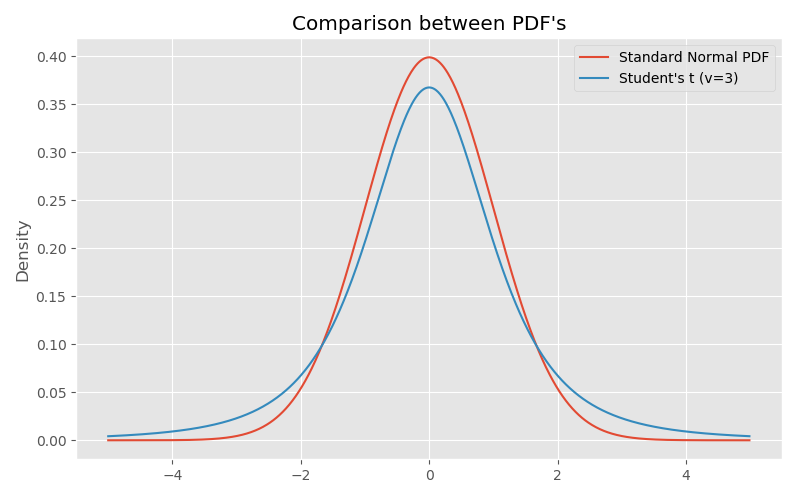
\includegraphics[scale=0.5]{images/normal_student_pdf.png}
\begingroup
\subcaption*{Parameters: the t-distributed variable has $\nu = 3$ df.}
\endgroup
\end{figure}

\subsection{1.2 Existence of moments}
As mentioned in the appendix, moments of $\nu - 1$ exist for a student's t-distributed variable $z_t$ with $\nu$ degrees of freedom.

\subsection{1.3 Log-likelihood function}
We are asked to find the log-likelihood function for the model given in (1.1)-(1.2). To do this, we first need to find the conditional moments. 

\subsubsection{1.3.1 Moments}
Given that $x_t$ is clearly Markov, we have the first two moments given by:
\begin{gather}
    \ee\lb x_t\vert x_{t-1}\rb 
        = \ee\lb \sqrt{\sigma^2 + \alpha x_{t-1}^2} z_t\vert x_{t-1}\rb
        = \sqrt{\sigma^2 + \alpha x_{t-1}^2}\ee\lb z_t\rb = 0\\
    \vv\lb x_t\vert x_{t-1}\rb
        = \lp \sigma^2 + \alpha x_{t-1}^2\rp \ee\lb z_t^2\rb = \sigma^2 + \alpha x_{t-1}^2.
\end{gather}

Notice, that the result above holds because $z_t$ has been scaled, as discussed in Appendix A.

\subsubsection{1.3.2 PDF}
With the conditional moments defined in equations (1.3) and (1.4), we next need to consider the conditional probability density function. With $z_t$ being t-distributed, we need the PDF for a t-distribution. 

We are told that the PDF is given by:
\begin{align}
    p\lp x \vert \nu, \mu, \sigma\rp 
        = \frac{\Gamma\lp \frac{\nu + 1}{2}\rp}{\Gamma \lp \frac{\nu}{2}\rp \sqrt{\pi\nu\sigma^2}}\lp 1 + \frac{1}{\nu}\lp \frac{x - \mu}{\sigma}\rp^2\rp^{-\frac{\nu + 1}{2}}
    \Rightarrow f\lp x\vert x_{t-1}\rp 
        = \frac{4}{\pi\sigma_t\lp 1 + z_t^2\rp^2},
\end{align}
where both the LHS and the RHS in (1.5) is derived in Appendix B.

\subsubsection{1.3.3 The log-likelihood function}
Taking the natural logarithm to (1.5) we find:
\begin{align}
    \ell_t\lp x_t \vert x_{t-1}\rp = \log\lp \frac{4}{\pi}\rp - \frac{1}{2}\log\lp \sigma_t^2\rp - 2\log\lp 1 + z_t^2\rp.
\end{align}

The result in (1.7) can itself be scaled and the constant removed, to attain:
\begin{align}
    \ell_t\lp \theta\rp = - \log\lp \sigma_t^2\rp - 4 \log \lp 1 + z_t^2\rp.
\end{align}

\subsection{1.4 Score}
Here we are given that the score $S_T$ evaluated at $\theta_0$ is given by:
\begin{align}
    \frac{1}{\sqrt{T}} S_T\lp \theta_0\rp
        = \frac{1}{\sqrt{T}}\sumt \frac{\partial \ell_t\lp \theta_0\rp}{\partial \alpha}
        = \frac{1}{\sqrt{T}}\sumt \frac{3z_t^2 - 1}{1 + z_t^2}\frac{x_{t-1}^2}{\sigma^2 + \alpha_0 z_{t-1}^2},
\end{align}

where a formal derivation can be found in appendix C.

We are asked to show, that the score in (1.8) is asymptotically Gaussian under appropriate conditions. We can show this, by applying theorem II.1, which is introduced below.

\begin{theorem}
Assuming theorem I.2 applies to $\lc X_t\rc_{t\geq 0}$, $X_t$ stationary. With $f\lp X_t, X_{t-1}, \dots, X_{t-m}\rp \in \rr$, assume that:
\begin{enumerate}
    \item $\ee\lb f\lp X_t, \dots, X_{t-m}\rp\vert X_{t-1}, \dots, X_{t-m}\rb = 0$
    \item $\ee\lb f^2\lp X_t, \dots, X_{t-m}\rp\rb < \infty$.
\end{enumerate}
In the case where assumptions (1) and (2) hold, the CLT applies as $T\rightarrow \infty$:
\begin{align}
    \frac{1}{\sqrt{T}}\sumt f\lp X_t, \dots, X_{t-m}\rp \overset{d}{\rightarrow} \nn\lp 0, \ee\lb f^2\lp X_t, \dots, X_{t-m}\rp\rb\rp.
\end{align}
\end{theorem}

Thus, for the score $f\lp X_t, \dots, X_{t-m}\rp = S_T\lp \theta_0\rp$ to be asymptotically Gaussian, we need to show that assumptions (1) and (2) in Theroem 1 apply to $S$, taking theorem 1.2 as given.

\subsubsection{1.4.1 Assumption 1}
With $x_t \vert x_{t-1}, \dots, x_{0} \overset{d}{=} x_t\vert x_{t-1}$, we consider the conditional expectation of $S_t$ given $x_{t-1}$, where each element in the sum of $S_T$ is denoted $S_t$, $t \in [1, T]$. 

First, we can define $y_t \equiv \frac{3z_t^2 - 1}{1 + z_t^2}$ and $f\lp z_{t-1}\rp = \xi_{t-1} \equiv \lp \frac{x_{t-1}}{\sigma_t}\rp^2 = \lp \frac{x_{t-1}}{\sigma^2 + \alpha x_{t-1}^2}\rp^2$, which depends on the shock $z_{t-1}$ and no other period shocks. That is $\xi_{t-1}$ is independent of $z_t$ for all $t$. Thus, we need to show that $\ee\lb y_t \xi_{t-1} \vert x_{t-1}\rb = 0$. We are told that $\ee\lb y_t\rb = 0$ (see Appendix D for derivation). Thus, applying the tower property we have:
\begin{align}
    \ee\lb y_t \xi_{t-1}\rb = \ee\lb \ee\lb y_t \xi_{t-1}\vert x_{t-1}\rb \rb = \ee\lb \xi_{t-1}\ee\lb y_t\vert x_{t-1}\rb \rb = \ee\lb \xi_{t-1}\ee\lb y_t\rb \rb = 0,
\end{align}
where the last equality follows from independence of $z_t$.

\subsubsection{1.4.2 Assumption 2}
We need to show that $\ee\lb \lp y_t \xi_{t-1}\rp^2\rb < \infty$. To do this, we first consider $\xi_t^2$:
\begin{align}
    \xi_t^2 = \frac{\sigma_{t-1}^4 z_{t-1}^4}{\lp \sigma^2 + \alpha \sigma_{t-1}^2z_{t-1}^2\rp^2} = \frac{\sigma_{t-1}^4 z_{t-1}^4}{\sigma^4 + \alpha^2 \sigma_{t-1}^4 z_t^4 + 2 \sigma^2 \alpha \sigma_{t-1}^2 z_{t-1}^2} < \frac{1}{\alpha}, \quad \alpha^2 > 0.
\end{align}

Applying (1.12) to the unconditional variance of the score elements, we find that:
\begin{align}
    \ee\lb \lp y_t \xi_{t-1}\rp^2\rb < \ee\lb y_t^2 \frac{1}{\alpha^2}\rb = \frac{1}{\alpha^2}\ee\lb y_t^2\rb < \infty.
\end{align}

We generally assume $\alpha> 0$ for return series, as this is the ARCH-effect which we are trying to capture and is itself the motivation of considering ARCH-models.

\subsubsection{1.4.3 Conclusion}
We verified that the conditions in Theorem 1 hold, specifically we showed in section (1.4.1) that condition (1) holds, and in (1.4.2) that condition (2) holds. Consequently the CLT applies to the score, such that it is asymptotically Gaussian.


\subsection{1.5}
In this question, we are asked to simulate 10,000 scores of t-ARCH series of lenght $T = 100$. Subsequently we will plot the QQ plots of the scores their corresponding density estimates. Plotting 10.000 realisations look as found in figure 2. Figure 3 shows the QQ-plot in the left panel and a histogram in the right panel. Remember that the asymptotic distribution is Gaussian, such that the histogram and QQ-plot compares to a Gaussian distribution.

\begin{figure}[ht]
\center
\caption{Realisations of scores}
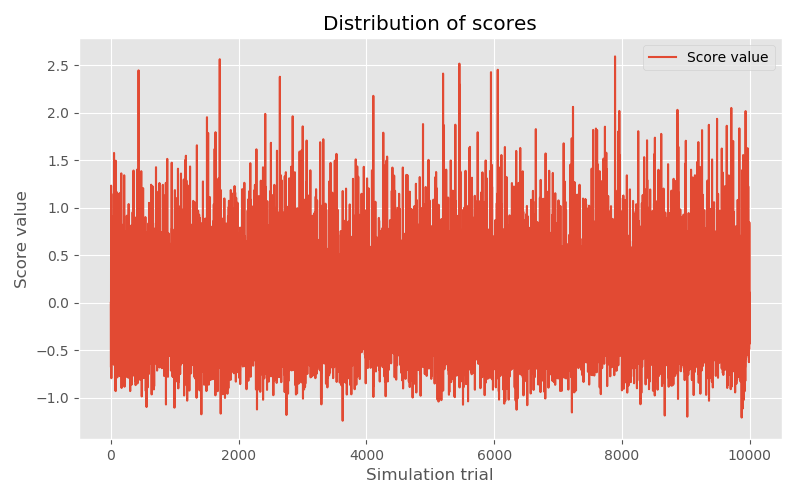
\includegraphics[scale=0.5]{images/score_simulation.png}
\begingroup
\subcaption*{Parameters: the t-distributed variable has been rescaled to have mean zero and unit variance. Df is 3.}
\endgroup
\end{figure}

As is clear from the charts in figures 2 and 3, the scores are not normally distributed. Because the theory states that the asymptotic distribution of the scores are Gaussian, I must look for the mistake in the simulation somewhere. The mean comes out seemingly correct, but there is a large right skew.

\begin{figure}[ht]
\centering
\captionsetup{justification=centering,margin=0.6cm}
\caption{Distribution of realised scores}
\begin{minipage}[b]{0.45\linewidth}
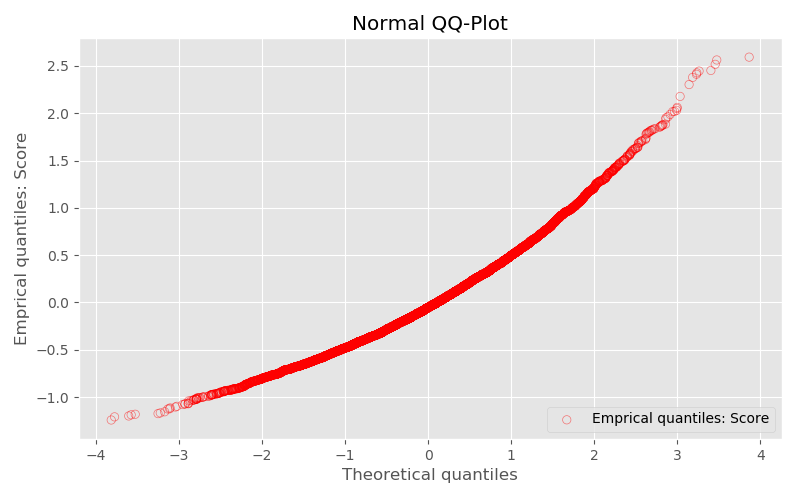
\includegraphics[scale = 0.45]{images/qq_score.png}
\end{minipage}
\hspace{0.5cm}
\begin{minipage}[b]{0.45\linewidth}
\centering
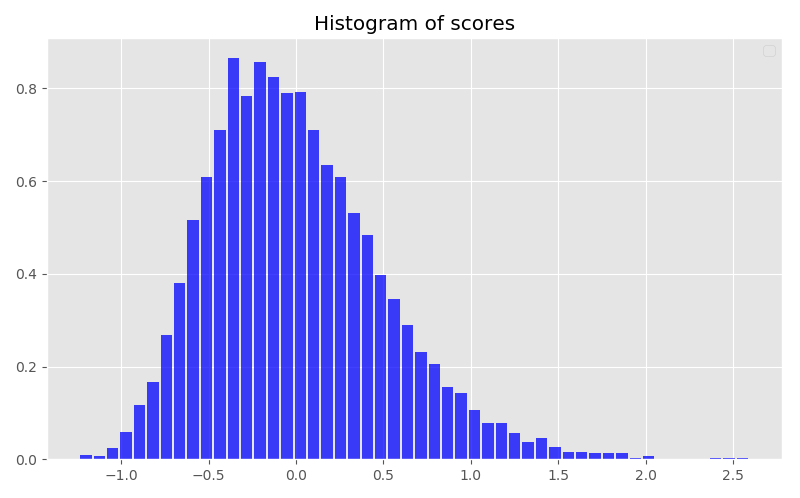
\includegraphics[scale = 0.45]{images/hist_scores.png}
\end{minipage}
\begingroup
\subcaption*{Parameters: the t-distributed variable has been rescaled to have mean zero and unit variance. Df is 3.}
\endgroup
\end{figure}

\subsection{1.6}
We showed in exercise 1.4 that the scores were asymptotically normal, which I did not manage to illustrate in exercise 1.5. Despite this, we accept the theoretical result.

Next, we consider the regularity conditions for the error $\hat \alpha - \alpha_0$ to be Gaussian. Here I refer to Theorem III.2 written below:
\begin{theorem}
We first assume that $\ell_T\lp \theta\rp$ is three times differentiable in $\theta$ with all derivatives continuous. With $\theta_0 \in \Theta$, we assume that:
\begin{enumerate}
    \item $\frac{1}{\sqrt{T}}S_T\lp \theta_0\rp = \frac{1}{\sqrt{T}}\frac{\partial \ell_T\lp \theta_0\rp}{\partial\theta} \overset{d}{\rightarrow} \nnn\lp 0, \Omega_S\rp, \quad \Omega_S > 0.$
    \item $\frac{1}{T}\lp \theta_0\rp = - \frac{1}{T}\frac{\partial^2 \ell_T\lp \theta_0\rp}{\partial\theta\partial\theta'}\overset{p}{\rightarrow}\Omega_I>0$
    \item $\max_{h,j,j=1, \dots, k}\sup_{\theta\in N\lp\theta_0\rp}\bigg\vert \frac{1}{T}\frac{\partial^3 \ell_T\lp \theta\rp}{\partial \theta_h\partial \theta_i \partial \theta_j}\bigg\vert \leq c_T$,
\end{enumerate}
where $N\lp \theta_0\rp$ is a neighbourhood around $\theta_0$, and $0\leq c_T \overset{d}{\rightarrow} c,$, $0 < c < \infty$.  Then, in a neighbourhood of $\theta_0$ abd as $T\rightarrow \infty$,
\begin{enumerate}
    \item $\hat \theta_T$, which solves the estimating equation, $\frac{\partial \ell_T\lp \hat \theta_T\rp}{\partial \theta} = 0$, is unique (with probability tending to one).
    \item $\hat \theta_T \overset{P}{\rightarrow} \theta_0$.
    \item $\sqrt{T}\lp \hat \theta_T - \theta_0\rp \overset{D}{\rightarrow} \nnn\lp 0, \Omega_I^{-1}\Omega_S\Omega_I^{-1}\rp$.
\end{enumerate}
\end{theorem}

Consider now a first-order Taylor-expansion of the score at the point $\theta = \theta_0$:
\begin{align}
    S_T\lp \hat \theta\rp 
        &\approx S_T\lp \theta_0 \rp + \frac{\partial S_T\lp \theta\rp}{\partial \theta}\bigg\vert_{\theta = \theta_0} \lp \hat \theta - \theta_0\rp + \dots  \notag \\
        &\approx S_T \lp \theta_0\rp - \iota_T\lp \theta_0\rp \lp \hat \theta - \theta_0\rp \notag \\
    \LL \sqrt{T}\lp \hat \theta - \theta_0\rp
        &\approx \lp \frac{1}{T}\iota_T\lp \theta_0\rp \rp^{-1} \frac{1}{\sqrt{T}}S_T\lp \theta_0\rp.
\end{align}

In practice the third assumption is rarely checked.

\subsection{Exercise 1.7}
We are now trying to fit the T-ARCH(1) model to the S\&P 500-index. To do this, we want to maximise the conditional log-likelihood function, which is the sum over all the contributions given in (1.7), i.e.:
\begin{align}
    \ell_T\lp \theta\rp = \sumt \ell_t \lp \theta \rp = - \sumt \lp \log\lp \sigma_t^2\rp + 4 \log \lp 1 + z_t^2\rp\rp.
\end{align}

We recall that maximising (1.14) is equivalent to minimising its negative, which is what we do in practice. Next, we choose $\theta = \lp \sigma^2 = 0.05, \alpha = 0.5\rp$ as starting values, leading to estimates and results as given in table 1 below.
\begin{table}[ht]
    \centering
    \caption{t-studen'ts ARCH(1) Maximum Likelihood results}
    \begin{tabular}{c|ccccc}  
    \toprule
                    & ML Estimate   &   SE      &   SE Robust   &   ML t-value  &   Robust t-value
    \\ \midrule
        $\sigma^2$  &  1.046543     &   0.04987 &   0.07121     &   20.98403    &   14.69684
    \\
        $\alpha$    &  0.288111     &   0.05388 &   0.07751     &   5.34679     &   3.716861
    \\ \midrule
    \end{tabular}
    \label{tab:ml_t_arch}
    \caption*{The maximisation returned a ML-value of 2,514.74316236.}
\end{table}

We not taht the estimated parameters are statistically significant regardless of which standard errors we use for computation. Treating the residuals as normal implies that we are running quasi maximum likelihood (QML) which is consistent, and is the reason why we usually consider standard normal residuals, rather than t-distributed noise.

\clearpage
\section{Exercise 2}
We consider here the GJR-ARCH(1) model given below:
\begin{align}
    x_t 
        &= \sigma_t z_t, \quad z_t \iid \nnn\lp 0, 1\rp, \\
    \sigma_t^2 
        &= \sigma^2 + \alpha x_{t-1}^2 + \gamma \ii_{\lc x_{t-1} < 0\rc} x_{t-1}^2, \quad \sigma^2 > 0, \quad \alpha, \gamma \geq 0.
\end{align}

\subsection{2.1 Comparison to A-ARCH and discussion}
This model is a reformulation of the asymmetric ARCH(1) model considered in week 4. To see this, write the following:
\begin{align}
    \sigma_{t, G}^2 = 
        \begin{cases}
            \sigma^2 + \lp \alpha + \gamma \rp x_{t-1}^2, & x_{t-1} < 0\\
            \sigma^2 + \alpha x_{t-1}^2, & x_{t-1} \geq 0
        \end{cases}\\
    \sigma_{t, A}^2 = 
        \begin{cases}
            \sigma^2 + \alpha_n x_{t-1}^2, & x_{t-1} < 0\\
            \sigma^2 + \alpha_p x_{t-1}^2, & x_{t-1} \geq 0
        \end{cases},
\end{align}

where the subscripts $G$ and $A$ refer to the GJR-ARCH and A-ARCH models, respectively. Thus, $\alpha_n \equiv \alpha + \gamma$ and $\alpha_p \equiv \alpha$.

In consequence, the interpretation is the same as for the A-ARCH model. The model allows for asymmetries in conditional variance, e.g. a negative shock may have a larger ARCH-effect on $\sigma_t^2$ than a positive shock. This effect is coined the "leverage effect".

\subsection{2.2 Log-likelihood function}
For this model, we note that there are three parameters to estimate, namely $\theta = \lp \sigma^2, \alpha, \gamma\rp$. The conditional moments of degrees one and two are given by:
\begin{gather}
    \ee\lb x_t \vert x_{t-1}\rb = 0, \quad \ee\lb x_t^2\vert x_{t-1}\rb = \sigma_t^2,
\end{gather}
with the process $\lc x_t\rc_{t\geq 1}$ being conditionally Gaussian distributed. Thus, the log-likelihood contributions are given by:
\begin{align}
    \ell_t\lp \theta\rp = \log\lp \frac{1}{\sqrt{2\pi\sigma_t^2}}\exp\lc - \frac{1}{2}\lp \frac{x_t}{\sigma_t}\rp^2\rc\rp = - \frac{1}{2}\lp \log\lp 2 \pi \sigma_t^2\rp + \lp\frac{x_t}{\sigma_t}\rp^2\rp,
\end{align}
with the conditional log-likelihood function given by:
\begin{align}
    \ell_T\lp \theta\rp = \sumt \ell_t.
\end{align}

\subsection{2.3 The score (not the album by the Fugees, unfortunately)}
We are asked to derive the score with respect to $\alpha$. This is given by the partial derivative below:
\begin{align}
    S_T^{\lp \alpha\rp}\lp \theta\rp = \frac{\partial \ell_T\lp \theta\rp}{\partial \alpha} 
        &= - \frac{1}{2}\sumt \lp \frac{x_{t-1}^2}{\sigma_t^2} - \frac{x_t^2}{\sigma_t^4}x_{t-1}^2\rp = - \frac{1}{2}\sumt \lp 1 - \frac{x_t^2}{\sigma_t^2}\rp \frac{x_{t-1}^2}{\sigma_t^2}.
\end{align}

\subsection{2.4 Asymptotic distribution of the score}
We are asked to discuss which assumptions are needed in order to have the score in (1.22) being asymptotically Gaussian distributed. We refer to theorem 1 above to emphasise the required assumptions. For the following derivations, we define by $f$ the elements in the score, i.e.:
\begin{align}
    f\lp x_t, x_{t-1}\rp = \lp 1 - z_t^2\rp \frac{x_{t-1}^2}{\sigma_t^2}.
\end{align}

\subsubsection{2.4.1 Assumption (i)}
The first assumption of a conditionally zero mean, is shown by:
\begin{align}
    \ee\lb f\lp x_t, x_{t-1}\rp \vert x_{t-1}\rb 
        = \ee\lb \lp 1 - z_t^2\rp \frac{x_{t-1}^2}{\sigma_t^2}\bigg \vert x_{t-1}\rb \notag 
        = \lp \ee\lb z_t^2 \rb - 1\rp \frac{x_{t-1}^2}{\sigma_t^2} 
        = 0,
\end{align}

where the second equality follows from $z_t$ being i.i.d. such that $\ee\lb z_t \vert x_{t-1} \rb = \ee\lb z_t\rb$.

\subsubsection{2.4.2 Assumption (ii)}
The second assumption is that of finite variance, which is shown as follows:
\begin{align}
    \ee\lb f^2\lp x_t, x_{-1}\rp \rb
        &= \ee\lb \lp \lp 1 - z_t^2\rp \frac{x_{t-1}^2}{\sigma_t^2}\rp^2 \rb \notag\\
        &= \ee\lb \lp z_t^4 + 1 - 2 z_t^2\rp \lp \frac{x_{t-1}}{\sigma_t}\rp^4\rb \notag \\
        &= \lp \ee\lb z_t^4\rb + 1 - 2\ee\lb z_t^2\rb \rp \ee\lb \lp \frac{x_{t-1}}{\sigma_t}\rp^4\rb \notag \\
        &= 2 \ee\lb \lp \frac{x_{t-1}}{\sigma_t}\rp^4\rb < \infty, \quad \alpha_0 > 0 \vee \ee\lb x_t^4\rb < 0,
\end{align}
where again the third equality follows from $z_t$ being i.i.d.

As these assumptions are shown to hold, we have that:
\begin{align}
    \frac{1}{\sqrt{T}}S_T\lp \theta_0 \rp \overset{d}{\rightarrow}\nnn\lp 0, \ee\lb f^2\lp x_t, x_{t-1}\rp\rb\rp.
\end{align}

\subsection{2.5 S\&P 500 estimation in the GJR-ARCH(1) framework}

Repeating the estimation steps in exercise 1.7 leads to the estimates in table 2 below.
\begin{table}[ht]
    \centering
    \caption{GJR Arch Maximum Likelihood results}
    \begin{tabular}{c|ccccc}  
    \toprule
                    &   ML Estimate &   SE      &   SE Robust   &   ML t-value  &   Robust t-value
    \\ \midrule
        $\sigma^2$  &   0.827574    &   0.05103 &   0.13355     &   16.21879    &   6.196656
    \\
        $\alpha$    &   0.360091    &   0.25919 &   0.81889     &   1.38931     &   0.439732
    \\
        $\gamma$    &   0.252586    &   0.82697 &   0.73821     &   0.88020     &   0.342158
    \\ \midrule
    \end{tabular}
    \label{tab:ml_gjr_arch}
    \caption*{The maximisation returned a ML-value of 2,029.17384396.}
\end{table}

Note that the estimates are highly unstable. In class we produced the estimates in table 3 below. Making an initial guess of $\theta = \lp 0.8, 0.05, 0.2\rp$ leads to the very same estimates to at least four decimals. Deviating too much from this initial guess will lead to other very different estimates.
\begin{table}[ht]
    \centering
    \caption{GJR Arch Maximum Likelihood results}
    \begin{tabular}{c|ccccc}  
    \toprule
                    &   ML Estimate &   SE      &   SE Robust   &   ML t-value  &   Robust t-value
    \\ \midrule
        $\sigma^2$  &   0.833698    &   0.03782 &   0.07550     &   22.04257    &   11.041992
    \\
        $\alpha$    &   0.062095    &   0.02829 &   0.04098     &   2.19150     &   1.515284
    \\
        $\gamma$    &   0.226405    &   0.07332 &   0.09670     &   3.08793     &   2.341301
    \\ \midrule
    \end{tabular}
    \label{tab:ml_gjr_arch_2}
    \caption*{The maximisation returned a ML-value of 2,005.915907.}
\end{table}

\subsubsection{Delta method}
I mentioned above that the solver was very sensitive to initial guess of parameters. This sensitivity can be decreased by transforming the parameters such that positive values are always achieved. The transformation is that of log:
\begin{align}
    \tilde \theta = \lp \log\lp \sigma^2\rp, \log \lp \alpha\rp, \log\lp \gamma\rp\rp' = \lp \tilde \sigma^2, \tilde \alpha, \tilde \gamma\rp'.
\end{align}

The log-likelihood function then becomes:
\begin{gather*}
    \ell_t\lp \tilde\theta\rp = -\frac{1}{2}\lc \log\lp 2\pi\rp + \log\lp \tilde \sigma_t^2\rp + \lp \frac{x}{\tilde \sigma_t}\rp^2\rc,\\
    \tilde \sigma_t^2 = \exp\lp \tilde \sigma^2\rp + \exp\lp \alpha\rp x_{t-1}^2 + \exp\lp \gamma\rp \ii_+ x_{t-1}^2.
\end{gather*}

By the sandwich method, we receive the standard errors belonging to $\tilde \theta$. To find the standard errors belonging to $\theta$, we have that:
\begin{align}
    \sqrt{T}\lp g\lp \hat{\tilde\theta}\rp - g\lp \tilde \theta\rp\rp \overset{d}{\rightarrow}\nnn\lp 0, g'\lp \tilde \theta\rp \tilde \Omega \lp g'\lp \tilde \theta\rp \rp^T\rp.
\end{align}

Because the transformation $g$ that helps us find the original parameters is the exponential function:
\begin{align*}
    g\lp \tilde \theta\rp = \exp\lp \tilde \theta\rp,
\end{align*}
we have that the matrix of derivatives $g' = A$ is given by:
\begin{align}
    g'\lp \tilde \theta\rp =
        \begin{pmatrix}
            \exp\lp \tilde \sigma^2\rp, & 0, & 0\\
            0, & \exp\lp \tilde \alpha^2\rp, & 0\\
            0, & 0, & \exp\lp \tilde \gamma^2\rp
        \end{pmatrix}.
\end{align}

Thus, the standard errors for $\theta$ are the square roots of the diagonals in $A \tilde \Omega A'$:
\begin{align}
    \Omega = A \tilde \Omega A'.
\end{align}

Doing these computations allow us to find the estimates and standard errors presented in table 3, without priming the initial guess. That is, with a wildly inaccurate guess, the estimation seems to still produce the "correct" results.









\clearpage


\section{Appendix A}
\renewcommand{\theequation}{A.\arabic{equation}}
\setcounter{equation}{0}

Consider an unscaled t-distributed random variable $z_t^0$ with $\nu > 3$ degrees of freedom. This has the following moments:
\begin{align}
    \ee\lb z_t^0\rb = 0, \quad \vv\lp z_t^0\rp = \frac{\nu}{\nu - 2}.
\end{align}

In general, $\nu - 1$ moments exist for a t-distributed random variable with $\nu$ degrees of freedom. To achieve the normalised t-distributed random variable $z_t$ in exercise 1, we have that:
\begin{align}
    z_t = z_t^0 \sqrt{\frac{\nu - 2}{\nu}}
\end{align}

This scaling implies that:
\begin{gather}
    \vv\lb z_t\rb
        = \vv\lb z_t^0\rb \frac{\nu - 2}{\nu}
        = \frac{\nu}{\nu - 2}\frac{\nu - 2}{\nu}
        = 1.
\end{gather}


\clearpage

\section{Appendix B}
\renewcommand{\theequation}{B.\arabic{equation}}
\setcounter{equation}{0}
Here we are deriving the PDF given in exercise 1.3.  We start by considering the PDF to $z_t$, which is t-distributed. In exercise 1 we consider a scaled $z_t$, but we first consider the unscaled case. Thereafter we adapt it to match the scaling of $z_t$.

The PDF is in general given by:
\begin{align}
    f\lp t\rp = \frac{\Gamma\lp \frac{\nu + 1}{2}\rp}{\sqrt{\nu \pi}\Gamma\lp \frac{\nu}{2}\rp}\lp 1 + \frac{t^2}{\nu}\rp^{-\frac{\nu + 1}{2}}.
\end{align}

Implementing a location parameter $\mu$ and a scale-parameter $\sigma$ such that a random variable $X$ is defined as:
\begin{align*}
    X_t = \mu + \sigma T,
\end{align*}
where $T$ is a t-distributed random variable, changes the PDF in (B.1) to:
\begin{align}
    p\lp x \vert \nu, \mu, \sigma\rp = \frac{\Gamma\lp \frac{\nu + 1}{2}\rp}{\Gamma \lp \frac{\nu}{2}\rp \sqrt{\pi\nu\sigma^2}}\lp 1 + \frac{1}{\nu}\lp \frac{x - \mu}{\sigma}\rp^2\rp^{-\frac{\nu + 1}{2}}.
\end{align}

It is (B.2) which is provided in the hint in exercise 1.3. Yet, we can do better still.

Finally, we must consider that $T$ has been rescaled, so that $\sigma^2 = \tilde \sigma^2 \frac{\nu - 2}{\nu}$, with $\mu = 0$ being unchanged. With these changes, we have that:
\begin{align*}
    f\lp x\rp = \frac{\Gamma\lp \frac{\nu + 1}{2}\rp}{\Gamma\lp \frac{\nu}{2}\rp\sqrt{\pi\lp \nu - 2\rp \sigma_t^2}}\lp 1 + \frac{1}{\nu - 2}\frac{x_t^2}{\sigma_t^2}\rp^{-\frac{\nu + 1}{2}}.
\end{align*}

With the $\Gamma$-function i.a. defined through:
\begin{align*}
    \Gamma\lp n\rp = \lp n - 1\rp!, \quad \Gamma \lp \frac{1}{2} + n\rp = \frac{\lp 2 n\rp !}{4^n n!}\sqrt{\pi},
\end{align*}

we have that for $\nu = 3$:
\begin{align}
    \Gamma\lp \frac{\nu + 1}{2}\rp = \Gamma \lp 2\rp = 2, \quad \Gamma \lp \frac{\nu}{2}\rp = \Gamma \lp \frac{1}{2} + 1\rp = \frac{2}{4}\sqrt{\pi} = \frac{1}{2}\sqrt{\pi}.
\end{align}

Thus, applying (B.4) to (B.3) we find:
\begin{align}
    f\lp x\vert x_{t-1}\rp 
        = \frac{2}{\frac{1}{2}\sqrt{\pi} \sqrt{\pi}\sigma_t}\lp 1 + z_t^2\rp^{-2}
        = \frac{4}{\pi\sigma_t\lp 1 + z_t^2\rp^2}.
\end{align}

\clearpage

\section{Appendix C}
\renewcommand{\theequation}{C.\arabic{equation}}
\setcounter{equation}{0}
This section shows a short derivation of the score provided in exercise 1.4. Here we were given that the score $S_T$ evaluated at $\theta_0$ is given by:
\begin{align*}
    \frac{1}{\sqrt{T}} S_T\lp \theta_0\rp
        = \frac{1}{\sqrt{T}}\sumt \frac{\partial \ell_t\lp \theta_0\rp}{\partial \alpha}
        = \frac{1}{\sqrt{T}}\sumt \frac{3z_t^2 - 1}{1 + z_t^2}\frac{x_{t-1}^2}{\sigma^2 + \alpha_0 z_{t-1}^2}.
\end{align*}

Recall that we found that the (transformed) log likelihood contributions were given by:
\begin{align}
    \ell_t\lp \theta\rp = - \log\lp \sigma_t^2\rp - 4 \log \lp 1 + z_t^2\rp.
\end{align}

Differentiating $\ell_t$ in (C.1) with respect to $\alpha$ at $\alpha = \alpha_0$ gives:
\begin{align}
    \frac{\partial \ell_t\lp \theta\rp}{\partial \alpha}\Bigg \vert_{\alpha = \alpha_0} 
        &= -\lp \frac{1}{\sigma_t^2}x_{t-1}^2 + 4 \frac{1}{1 + z_t^2}\lp - \frac{x_t^2}{\sigma_t^4}\rp x_{t-1}^2\rp \notag \\
        &= 4 \lp \frac{x_{t-1}}{\sigma_t}\rp^2 z_t^2\frac{1}{1 + z_t^2} - \lp \frac{x_{t-1}}{\sigma_t}\rp^2\notag\\
        &= \lp \frac{x_{t-1}}{\sigma_t}\rp^2\lp \frac{4 z_t^2}{1 + z_t^2} - 1\rp\notag \\
        &= \lp \frac{x_{t-1}}{\sigma_t}\rp^2\frac{4 z_t^2 - \lp 1 + z_t^2\rp}{1 + z_t^2}\notag\\
        &= \lp \frac{x_{t-1}}{\sigma_t}\rp^2 \frac{3 z_t^2 - 1}{1 + z_t^2}.
\end{align}

It is the result in (C.2) that yields the score in (1.8).

\clearpage 

\section{Appendix D}
\renewcommand{\theequation}{D.\arabic{equation}}
\setcounter{equation}{0}
In question 1.4 we are told that $\ee\lb y_t\rb = 0$ and that $\ee\lb y_t^4 \rb < \infty$. We first show the first moment, with a referral to \cite{PedersenRahbek} as the source for the proof.

\subsection{D.1 Zero expectation}
In a general setting, we define:
\begin{align}
    y_t = \lp \nu + 1 \rp \frac{z_t^2}{\lp \nu - 2\rp + z_t^2} - 1,
\end{align}
and we note that for $\nu = 3$ we have that $y_t = \frac{4 z_t^2}{1 + z_t^2} - 1 = \frac{4 z_t^2 - \lp 1 + z_t^2\rp}{1+ z_t^2} = \frac{3 z_t^2 - 1}{1 + z_t^2}$ as given in problem 1.4. Next, define:
\begin{align}
    \eta_t = \frac{z_t^2}{\lp \nu - 2\rp + z_t^2} \in [0, 1[.
\end{align}

By Johnson, Kempt and Kotz (1995) \cite{johnson1995continuous}, we have that:
\begin{align}
    \eta \sim \text{Beta}\lp \frac{1}{2}, \frac{\nu}{2}\rp,
\end{align}

where a Beta-distributed random variable $X \sim \text{Beta}\lp p, q\rp$ has expectation $\ee\lb X\rb = \frac{p}{p + q}$. Thus, noting that $y_t$ in (D.1) can be written as a function of $\eta_t$ as defined in (D.2) rather than $z_t$:
\begin{align}
    y_t = \lp \nu + 1\rp \frac{z_t^2}{\nu - 2 +z_t^2} - 1 = \lp \nu + 1\rp \eta_t - 1,
\end{align}

we have that $\ee\lb y_t\rb$ is given by:
\begin{align}
    \ee\lb y_t\rb = \lp \nu + 1\rp \ee\lb \eta_t\rb - 1 = \lp \nu + 1\rp \frac{\frac{1}{2}}{\frac{1 + \nu}{2}} - 1 = \frac{\nu + 1}{\nu + 1} - 1 = 0, \quad \forall \nu > 2.
\end{align}

The result in (D.5) shows the desired result.

\subsection{D.2 Finite variance}
Next, we want to show that the second moment is finite. More specifically, Pedersen and Rahbek (2016) show that $\ee\lb y_t^2\rb = \frac{2\nu}{\nu + 3}< \infty$, for $\nu \geq 3$. We will apply the fact that $\ee\lb X^2\rb = p \lp p + q\rp^{-1} \lp p + 1\rp \lp p + q + 1\rp^{-1}$ for $X \sim \text{Beta}\lp p, q\rp$.

Recall the distribution stated in (D.3) and consider the variance of $y_t$ as defined in (D.4):
\begin{align}
    \vv\lp y_t\rp = \ee\lb y_t^2 \rb 
        &= \ee\lb \lp  \lp 1 + \nu \rp \eta_t - 1 \rp^2\rb \notag \\
        &= \ee\lb \lp 1 + \nu\rp^2\eta_t^2 + 1 - 2 \lp 1 + \nu\rp \eta_t\rb \notag\\
        &= \lp 1 + \nu\rp^2 \ee\lb \eta_t^2\rb + 1 - 2\lp 1 + \nu\rp \ee\lb \eta_t\rb\notag\\
        &= \lp 1 + \nu\rp^2 \lp \frac{1}{2}\frac{2}{1 + \nu}\frac{1 + 2}{2}\frac{2}{1 + \nu + 2}\rp + 1 - 2 \lp 1 + \nu\rp \frac{1}{1 + \nu}\notag\\
        &= \frac{3 \lp 1 + \nu\rp}{3 + \nu} -1\notag\\
        &= \frac{3 + 3\nu - \lp 3 + \nu\rp }{3 + \nu}\notag\\
        &= \frac{2\nu}{3 + \nu} < \infty.\notag
\end{align}

The result in (D.6) is what we wanted to show.

\clearpage

\section{Bibliography}
\printbibliography[heading=none]

\end{document}